\documentclass{cmn}

\newcommand\width{20mm}
\newcommand\sep{5mm}
\newcommand\labely{-10mm}

\begin{document}
  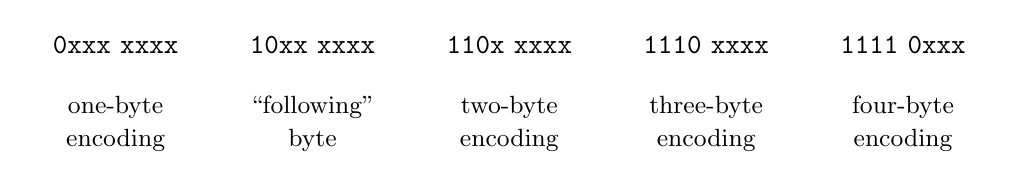
\begin{tikzpicture}
    \node[text width=\width,align=center] at (0,0) {\texttt{0xxx xxxx}};
    \node[text width=\width,align=center] at (\width+\sep,0) {\texttt{10xx xxxx}};
    \node[text width=\width,align=center] at (2*\width+2*\sep,0) {\texttt{110x xxxx}};
    \node[text width=\width,align=center] at (3*\width+3*\sep,0) {\texttt{1110 xxxx}};
    \node[text width=\width,align=center] at (4*\width+4*\sep,0) {\texttt{1111 0xxx}};

    \node[text width=\width,align=center] at (0,\labely) {\small one-byte\\ encoding};
    \node[text width=\width,align=center] at (\width+\sep,\labely) {\small ``following''\\ byte};
    \node[text width=\width,align=center] at (2*\width+2*\sep,\labely) {\small two-byte\\ encoding};
    \node[text width=\width,align=center] at (3*\width+3*\sep,\labely) {\small three-byte\\ encoding};
    \node[text width=\width,align=center] at (4*\width+4*\sep,\labely) {\small four-byte\\ encoding};
  \end{tikzpicture}
\end{document}
